%\documentclass[10pt,slidesonly,semrot,portrait,palatino]{seminar}
%style{200t}{\\Principles of Biostatistics \hfil}{\thepage}

%%%% For four on a page:
%\documentclass[10pt,2up,article,semrot,palatino]{seminar}
%\pagestyle{empty}
%\articlemag{0}
%\twoup[1]
%style{200t}{\\Principles of Biostatistics \hfil}{}
%\pagestyle{200t}
%\slidepagestyle{200t}
%\renewcommand{\printlandscape}{\special{landscape}}
\documentclass[10pt]{book}
\newcommand{\bfZ}{\mathbf{Z}}
\newcommand{\bfbeta}{\mathbf{\beta}}
\newcommand{\bfI}{\mathbf{I}}
\usepackage{amssymb}
\usepackage{amsmath}
\usepackage{epsfig}
\usepackage{euscript}
%\rotateheaderstrue
%\slideframe{plain}
%\setlength{\slideframewidth}{1pt}
%\onlyslides{1-2}

\begin{document}\setcounter{chapter}{8}\setcounter{page}{141}
\chapter{Time-dependent covariates}
In many situations it is useful to consider covariates that change over time.  These are called
``time-dependent" covariates.  Such are of two kinds:
\begin{enumerate}
\item Internal variables\\
These are related to each patient and are measurable while the patient is under observation
\item External variables\\
These are variables that do not depend on the physical observation of the patient such as
\begin{enumerate}
\item Variables such as age that are known once the birth date or age at enrollment to the study is known
\item Variables that are independent of any individual like levels of pollution or temperature
\end{enumerate}
\end{enumerate}
These time-updated or dependent variables can be entered into the Cox model in direct extension of the
simpler non-time-updated case
$$
\lambda_i(t;\bfZ_i)=\lambda_0(t)\exp{\sum_{j=1}^n\beta_jZ_{ij}(t)}
$$
where $\lambda_0(t)$ is the baseline hazard associated with all covariates being equal to zero {\it during all
time points $t$}.  So the Cox model is generalized as
$$
\sum_{i=1}^n\delta_i\left \{ \sum_{j=1}^p\beta_jZ_{ij}(t_i)-\log\sum_{l\in R(t_i)}\exp\left (
\sum_{j=1}^p\beta_jZ_{jl}(t_i)\right )\right \}
$$
this means that we will need to have all the variable (especially internal ones) available at each event time.  It is important to understand that this is no longer a proportional hazards model.
\\[2ex]
When the value of a time-updated covariate is not known during a failure time $t$ we can use various methods to fill in a value for a particular time (see figure below).  We can either extend the most recent value or, if two values  are available on either side of the time point we can use interpolation.
\begin{figure}[ht]
\centerline{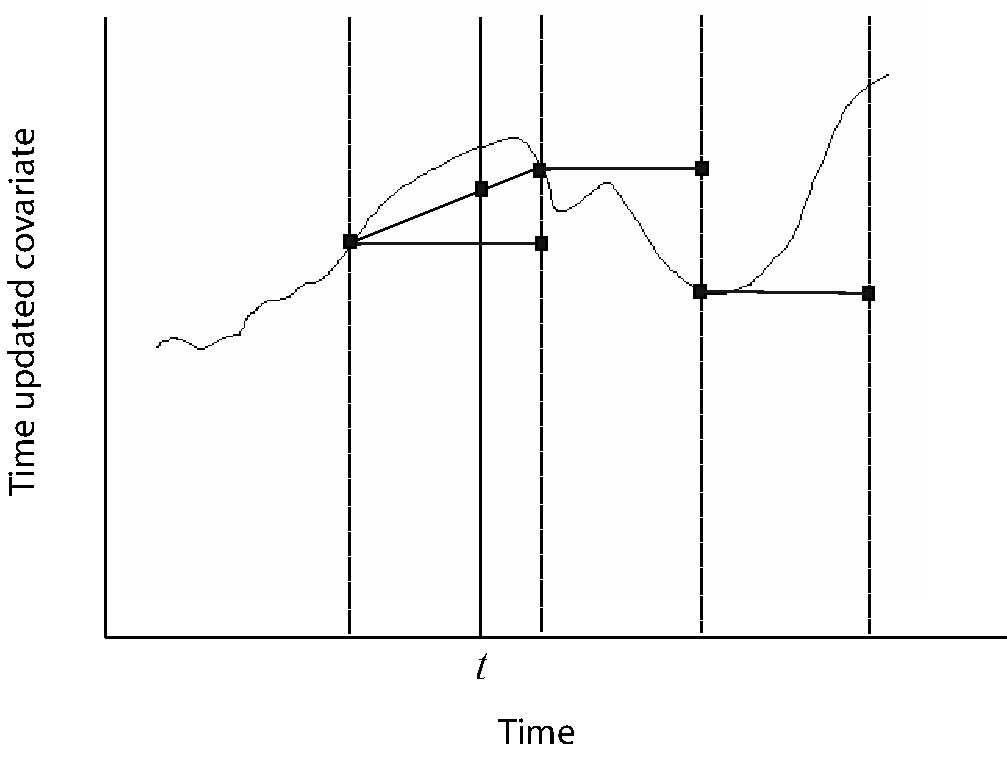
\includegraphics[width=3in]{lect8_g1.pdf}}
\caption{Time updated covariates}
\end{figure}
\section{The Stanford heart transplant data}
We present here the famous Stanford heart transplant data set (Crowley \& Hu, 1977).  In this data set, 103 individuals waiting for a heart transplant were followed for survival.  The problem that the study presented to the original investigators (and us) is that the effect of heart transplantation on survival is impossible to assess given the methods that we have been exposed to.\\
\\[2ex]
The reason is that the hazard of an individual is different before and after a transplantation and, for an individual to receive a transplant, they have to have survived up to the point that an organ is available.  As Collett describes the situation (Section 7.3), the two groups are also not comparable at the time origin (entry into the study and time from transplantation).\\[2ex]
Before considering the correct analysis, let's perform a naive analysis involving a conventional PH model
\\[2ex]
This analysis indicates that transplantation is associated with one quarter of the hazard compared to no transplantation.\newpage
\small
\begin{verbatim}
Call:
coxph(formula = Surv(time, fail) ~ transplant, data = stanford)

  n= 103, number of events= 75

              coef exp(coef) se(coef)     z Pr(>|z|)
transplant -1.3238    0.2661   0.2438 -5.43 5.63e-08 ***
---
Signif. codes:  0 ‘***’ 0.001 ‘**’ 0.01 ‘*’ 0.05 ‘.’ 0.1 ‘ ’ 1

           exp(coef) exp(-coef) lower .95 upper .95
transplant    0.2661      3.758     0.165    0.4291

Concordance= 0.668  (se = 0.026 )
Rsquare= 0.223   (max possible= 0.997 )
Likelihood ratio test= 25.96  on 1 df,   p=3.481e-07
Wald test            = 29.49  on 1 df,   p=5.627e-08
Score (logrank) test = 33.41  on 1 df,   p=7.463e-09
\end{verbatim}
\normalsize
Given the misgivings about the appropriateness of the comparison, the solution is to introduce a time-updated covariate $Z(t)$ so that
$$
Z(t)=\left \{ \begin{array}{c}
  1,\mbox{if } t>T_o \\
  0,\mbox{if } t\leq T_o\\
\end{array}\right .
$$
where $T_o$ is the time of transplantation.\\[2ex]
Crowley and Hu suggest that the hazard associated with this situation is
$$
\lambda_i(t_i;\bfZ_i)=\lambda_0(t)\exp\left \{ \eta_i+\beta_1Z_{1i}(t)\right \}
$$
where $\eta_i$ is the summation of the products of all other covariates and their associated coefficients (excluding $Z_{1i}(t)$) measured on each individual $i$ at each time $t$.
\\[2ex]
The hazard ratio (according to Crowley and Hu, 1977) is
$$
\frac{\lambda(t_i;\bfZ_1(t))}{\lambda(t_i;\bfZ_0(t))}=\left \{ \begin{array}{c}
   \lambda_0(t)\exp\left \{ \eta_i\right \}\mbox{, before tranplantation}\\
  \lambda_0(t)\exp\left \{ \eta_i+\beta_1 \right \}\mbox{, after tranplantation}\\
\end{array}\right .
$$
If $\beta_1<0$ then the hazard ratio of two individuals (one without a transplant and one with one) looks as follows (where $T_0$ is the time of transplantation:
\begin{figure}[ht]
\centerline{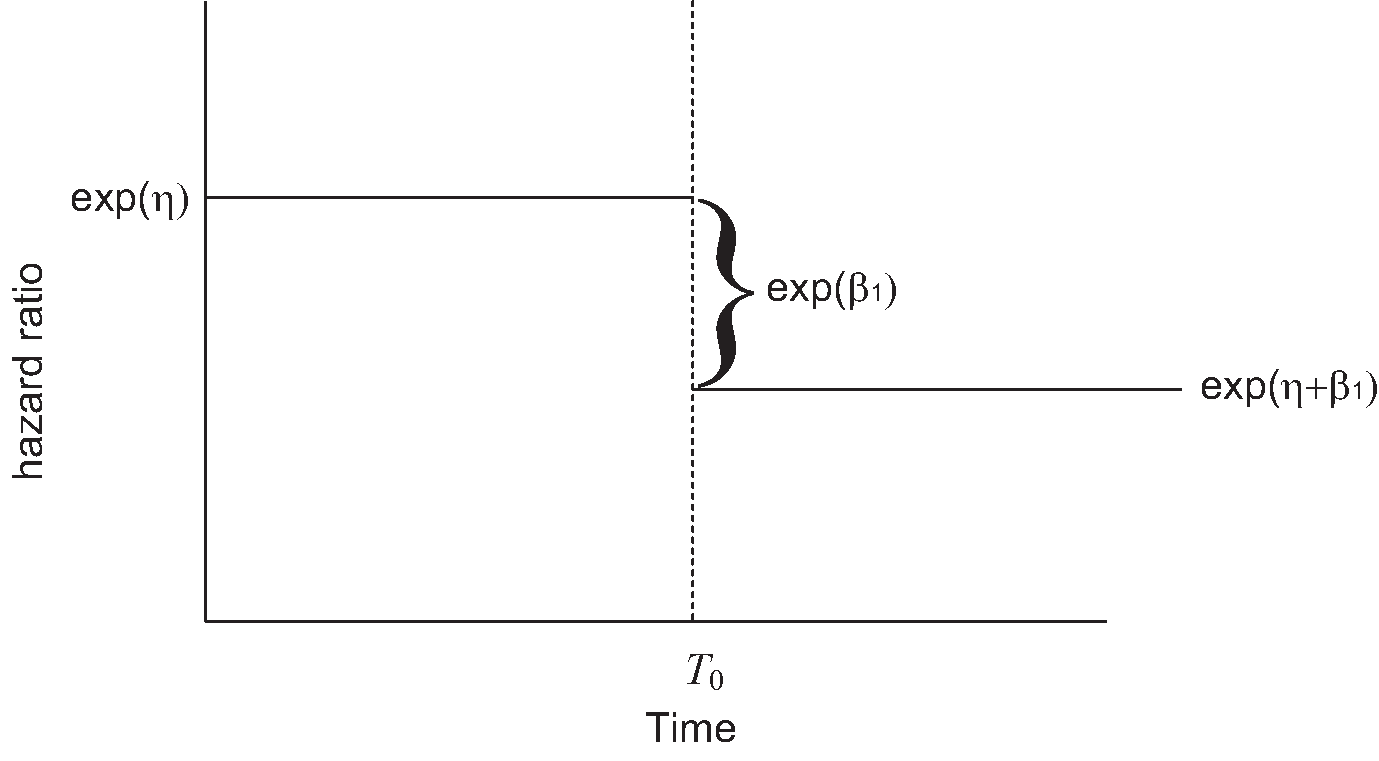
\includegraphics[width=4in]{lect8_g2.pdf}}
\caption{Analysis with a simple time updated covariate}
\end{figure}
In the original analysis, the effect of transplantation on the hazard is assessed by testing the significance of the coefficient $\beta_1$.\\
\\[2ex]
The null hypothesis $H_0: \beta_1=0$ suggests that there is no effect on survival resulting from transplantation. On the other hand, the alternative hypothesis $H_A: \beta_1<0$ suggests a beneficial effect of the transplantation, while the alternative $H_A: \beta_1>0$ suggests a detrimental effect (increase in hazard of death) conferred by tranplantation.

\section{Cox \& Oakes' reanalysis of the heart transplant data}
The previous model does not account for the fact that a heart tranplantation is a delicate and very dangerous operation.  Thus, even if the hazard is ultimately reduced from the pre-transplant levels, a period of very high hazard is likely to follow the operation.  Cox and Oakes (1984) improve on the analysis of Crowley and Hu by introducing factors $\beta_2$ and $\beta_3$ as follows:
$$
\lambda_i(t_i;\bfZ_i)=\lambda_0(t)\exp\left \{ \eta_i+\beta_1+\beta_2\exp[-\beta_3(t-T_0)]\right \}
$$
The hazard ratio is
$$
\frac{\lambda(t_i;\bfZ_1(t))}{\lambda(t_i;\bfZ_0(t))}=\left \{ \begin{array}{l}
   \lambda_0(t)\exp\left \{ \eta_i\right \}\mbox{, before tranplantation}\\
   \lambda_0(t)\exp\left \{ \eta_i+\beta_1+\beta_2 \right \}\mbox{, right at tranplantation}\\
   \lambda_0(t)\exp\left \{ \eta_i+\beta_1\right \}\mbox{, asymptotically (i.e., at $t\rightarrow\infty$})\\
\end{array}\right .
$$
The Cox \& Oakes reanalysis results in a hazard ratio that looks graphically as follows:
\begin{figure}[ht]
\centerline{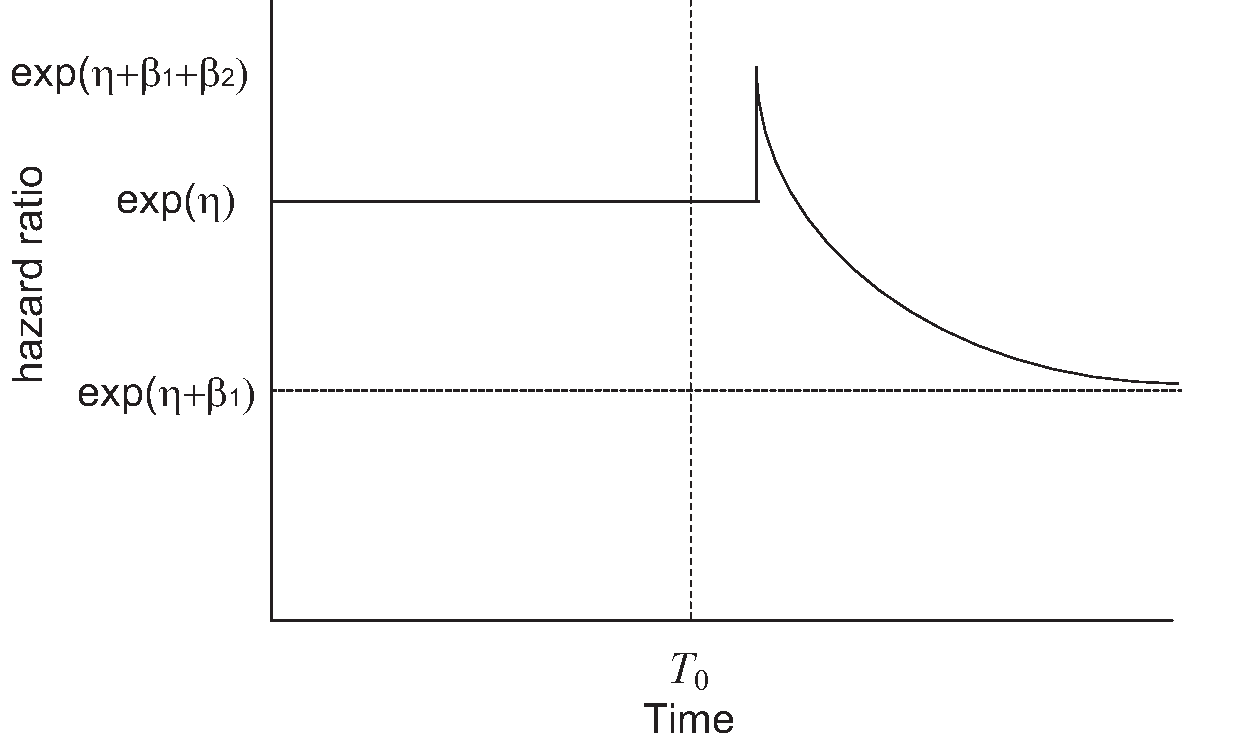
\includegraphics[width=4in]{lect8_g3.pdf}}
\caption{The Cox \& Oakes analysis of the Stanford heart transplant data}
\end{figure}
\subsection{Notes}
\begin{itemize}
\item
In the reanalysis of Cox \& Oakes, the effect of transplantation on the hazard is assessed by a more complex procedure.
\item A large positive $\beta_3$ suggests a steep decrease of the hazard from an original level, just after transplantation, of $\exp(\eta_i+\beta_1+\beta_2)$ to a level $\exp(\eta_i+\beta_1)$.  A large positive value of $\beta_2$ suggests a large temporary increase of the hazard ratio post-transplantation.  Conversely a smaller value of $\beta_2$ suggests small or negligible such increases.
\item
The latter asymptote ($\exp(\eta_i+\beta_1))$ depends on the magnitude and sign of $\beta_1$.  The previous comments apply. That is, a large negative $\beta_1$ suggests a significant survival decrease (eventually) post tranplantation. \item
Note that the Cox \& Oakes model is equivalent to the Crowley \& Hu model if $\beta_2=0$.  The disadvantage of this model is that it requires specialized software to fit it.
\end{itemize}
\normalsize
To perform any analysis involving the time-updated transplant status, we need to create two lines (one pre-transplantation and one post-transplantation) for the patients that received a transplant.  Thus, the line for patient 95 for example in the original data set is

\small
\begin{verbatim}
     patid  year  age  fail     time  surgery  transplant    waitime   
95      95    73    40    1       16        0           1          2 
\end{verbatim}
\normalsize
where \textsf{waitime} is the waiting time to transplantation.  The data for this patient will be recoded as follows:
\small
\begin{verbatim}
     patid  year  age  fail     time  surgery  transplant   waitime   ord
95      95    73    40    1       16        0           1         2     1
95.1    95    73    40    1       16        0           1         2     2
\end{verbatim}
\normalsize
in other words, we introduce a second line copying all data for this patient.
\subsection{The counting process approach to survival analysis}
A general approach to survival analysis was introduced by Andersen \& Gill (1982) where each subject is considered as a counting process (counting events).
\begin{itemize}
\item $N_i(t)$ is the total number of events for each subject $i$ up to time $t$
\item $Y_i(t)$ is an indicator function with $Y_{i}(t)=1$ if subject $i$ is at risk at time $t$ for the event
\end{itemize}
In this formulation the hazard is considered as an ``intensity" process such that
$$
\lambda_i(t)=Y_i(t)\lambda_0(t)\exp\{\beta'Z_i\}
$$
By judicious choice of the various components of the process as defined above, the counting process approach can handle all kinds of survival data including
\begin{itemize}
\item Time updated covariates $Z_i(t)$
\item Discontinuous risk sets
\item Multiple events of the same or different type\\
Here we replace $N_i(t)$ , $Y_i(t)$ and $\lambda_0(t)$ by $N^{(k)}_i(t)$ , $Y^{(k)}_i(t)$ and $\lambda^{(k)}_0(t)$
respectively for each event of type $k$ (we will see more of that in a future lecture).  By doing so, we can handle
\begin{itemize}
\item Multiple failures of the different type (competing risks)
\item Multiple failures of the same type (both ordered and unordered)
\end{itemize}
\end{itemize}
\subsection{R analysis of the Crowley \& Hu data}
Let's return to  the previous patient \# 95. During the waiting time, $\delta_i=0$ since no failure has occurred, and $Z_1(t)=0$ since a transplantation has not taken place. Thus, we will set {\tt fail=0} and {\tt transplant=0} in the first line.
\\[2ex]
In tthe second line (post-transplantation period) $\delta_i$ is set to whatever the failure status of the patient is (in this case the patient died under observation, so $\delta_i=1$).  Also $Z_i(t)=1$ here since the patient has received a transplantation.
\\[2ex]
We also generate two new variables named {\tt tstart} and {\tt tsttop}. In the first line, we are covering the interval prior to transplantation (i.e., the interval $[0,2)$), so {\tt tstart=0} (in fact, {\tt tstart=0} always in the first interval) and {\tt tstop=waitime}.  In the second interval, which is associated with the time interval $[2,16)$ i.e, the 14 months of post-transplantation survival, {\tt tstart=waitime} and {\tt tstop=time} (in fact, in the final interval of every subject, whether this is the first interval for those without transplant or the second interval for those with a transplant, {\tt tstop} is always equal to {\tt time}).\\[2ex]
A situation arises with patient 38, who died on the same day of the transplantation (so \textsf{waitime}=\textsf{survtime}).
\small
\begin{verbatim}
    patid   year  age  fail  time  surgery  transplant  waitime  
38     38    70    41    1      5        0           1        5  
\end{verbatim}
\normalsize
Since this would cause most statistical software to exclude this case from consideration, we add a small fraction to the survival time (i.e., we assume that the patient lived a short time after receiving transplantation).  This patient's data will look as follows:
\small
\begin{verbatim}
    patid  year  age  fail    time   surgery  transplant  waitime  ord
38     38    70    41    0       5         0           0        5    1
38.1   38    70    41    1     5.1         0           1        5    2
\end{verbatim}
\normalsize
In the same manner we are defining a starting ({\tt tstart)} and stopping time ({\tt tstop}) for each line of data for each patient:
\small
\begin{verbatim}
     patid year age fail  time surgery transplant waitime ord tstop tstart
12      12   68  53    1   8.0       0          0      NA   1   8.0      0
16      16   68  56    0  43.0       0          0      20   1  20.0      0
16.1    16   68  56    1  43.0       0          1      20   2  43.0     20
38      38   70  41    0   5.1       0          0       5   1   5.0      0
38.1    38   70  41    1   5.1       0          1       5   2   5.1      5
80      80   72  46    0 482.0       1          0      26   1  26.0      0
80.1    80   72  46    0 482.0       1          1      26   2 482.0     26
\end{verbatim}
\normalsize
Notice that the starting time in the first line for each patient (including those without transplant) is zero.  \\[2ex]
For those with a transplant (and, thus, having a second line of data) the ending time of the first interval is {\tt waitime} and the starting time of the interval is the end of the previous interval (identical to {\tt waitime}).
\\[2ex]
The R analysis of the Crowley \& Hu model with only transplantation as the covariate is as follows (notice the new syntax within the {\tt Surv} command):

\small
\begin{verbatim}
Call:
coxph(formula = Surv(tstart, tstop, fail) ~ transplant, data = stanford2)

  n= 172, number of events= 75

             coef exp(coef) se(coef)     z Pr(>|z|)
transplant 0.1067    1.1126   0.2984 0.357    0.721

           exp(coef) exp(-coef) lower .95 upper .95
transplant     1.113     0.8988    0.6199     1.997

Concordance= 0.509  (se = 0.025 )
Rsquare= 0.001   (max possible= 0.969 )
Likelihood ratio test= 0.13  on 1 df,   p=0.7198
Wald test            = 0.13  on 1 df,   p=0.7207
Score (logrank) test = 0.13  on 1 df,   p=0.7207

\end{verbatim}
\normalsize
{\bf Comments:}
\\[2ex]
The estimate of $\beta_1$ is $\hat\beta_1=0.1067$ associated with a hazard ratio
of $e^{\beta_1}=1.113$.
\\[2ex]
The interpretation is that transplantation increases slightly the hazard for death  (by about
11\%), an increase that is not statistically significant (p=0.720). The log hazard ratio represented by $\beta_1$ concerns the comparison between a person that has undergone transplantation and one that has not.
\section{Checking the PH assumption via time-updated covariates}
As noted earlier, we can check the PH assumption by introducing an interaction between the effect and time
\[   \lambda(t; Z)  = \lambda_0(t) ~ \exp\{\beta_1 Z_1 + \cdots + \beta_p Z_p + \gamma Z_1*t\} \]
... or carrying out a stratified analysis
\[   \lambda(t; Z)  = \lambda_{0,Z_1}(t) ~ \exp\{\beta_2 Z_2 + \cdots + \beta_p Z_p\} \]
where $\lambda_{0,Z_i}(t)$ are baseline hazards over all levels of $Z_1$.\\[2ex]
Notice that these are different analyses: In the first case we impose a \textit{linear} change (increase or decrease depending on the sign of $\gamma$) on the hazard ratio over time, while, in the second case, the change of the baseline hazard over time in the various levels of $Z_1$ can be arbitrary.\\[2ex]
We will focus here on the first case.
\subsection{Re-analysis of the leukemia data set}
Consider the check on the proportionality assumption in the case of the leukemia data.
\begin{figure}[h!]
\caption{Log-log plot in the leukemia data set example}
\centerline{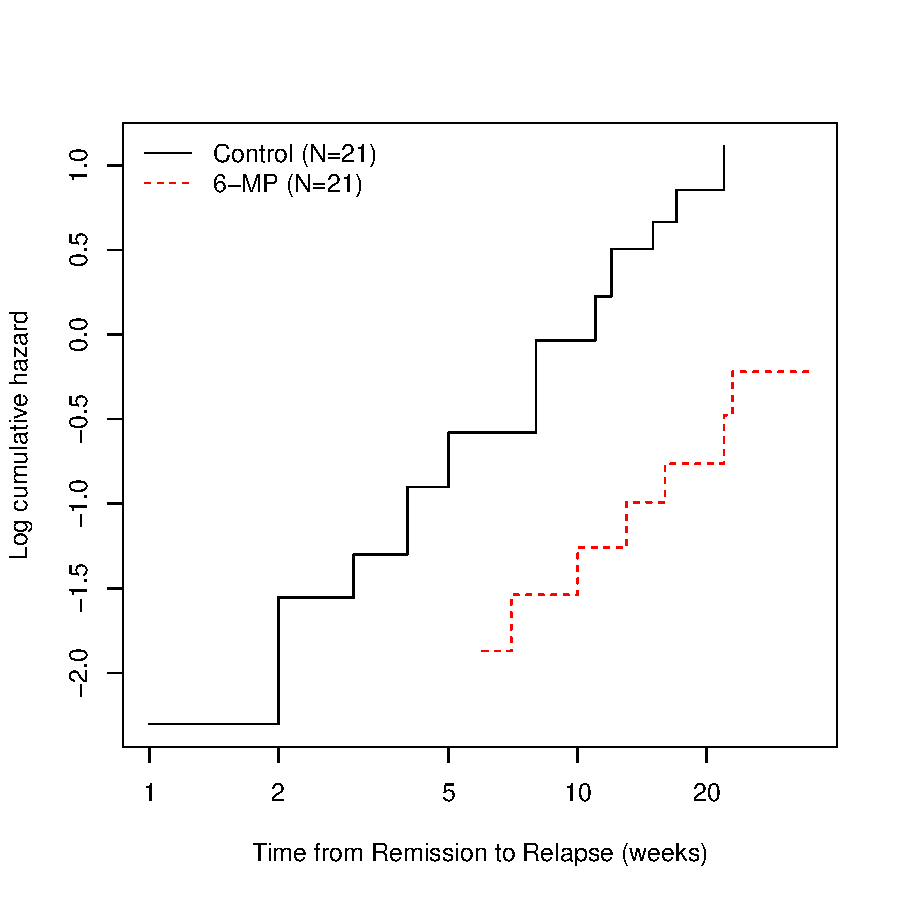
\includegraphics[width=3in]{leukemlogHaz.pdf}}
\end{figure}
\newpage\noindent
Even though the PH assumption appears to be fulfilled in this case, we will analyze the data by introducing a time-treatment interaction:

\small
\begin{verbatim}
Call:
coxph(formula = Surv(weeks, remiss) ~ trt + I(weeks * (trt ==
    "6-MP")), data = leukem)

  n= 42, number of events= 30

                               coef exp(coef) se(coef)      z Pr(>|z|)
trtControl                 -1.47927   0.22780  0.81291 -1.820 0.068800 .
I(weeks * (trt == "6-MP")) -0.18138   0.83412  0.05479 -3.311 0.000931 ***
---
Signif. codes:  0 ‘***’ 0.001 ‘**’ 0.01 ‘*’ 0.05 ‘.’ 0.1 ‘ ’ 1

                           exp(coef) exp(-coef) lower .95 upper .95
trtControl                    0.2278      4.390    0.0463    1.1207
I(weeks * (trt == "6-MP"))    0.8341      1.199    0.7492    0.9287

Concordance= 0.773  (se = 0.06 )
Rsquare= 0.534   (max possible= 0.988 )
Likelihood ratio test= 32.11  on 2 df,   p=1.066e-07
Wald test            = 15.19  on 2 df,   p=0.0005029
Score (logrank) test = 25.11  on 2 df,   p=3.532e-06

\end{verbatim}
\normalsize
{\bf Comments:}\\[2ex]
Here we have $\gamma=-0.18138$, which is statistically significant.  The interpretation is that the hazard ratio is \textit{decreasing} linearly over time (in favor of 6-MP).\\[2ex]
This is a surprising result given the previous figure, particularly given how strong this deviation from proportionality appears to be. (An almost 17\% reduction in the hazard ratio \textit{at each unit in time} above and beyond the overall four-fold reduction experienced by individuals treated with 6-MP).\\[2ex]
In turn, this means that treatment with 6-MP has an accumulating benefit to the patient which increases over time.\\[2ex]
{\bf Unfortunately, this is wrong!}
\\[2ex]
Why was this the wrong analysis?\\[2ex]
The previous model was wrong for the following reason:  It inserted as a covariate for time the entire follow-up time for each patient!\\[2ex]
So, even for risk sets involving failure times $\tau_j<T_i$, for the other subjects with $T_j<T_i$, the model, as structured, inserts the entire $T_i$ as a covariate.\\[2ex]
The correct analysis involves breaking up each $T_i$ into each $\tau_j$ up to $T_i$ and carrying out a time-updated analysis, similar to the one in the Crowley \& Hu dataset, with {\tt tstart} each failure time $\tau_j$ and {\tt tstop} the next ranked failure time $\tau_{j'}$ up to $T_i$. \\[2ex]
In R, this is done by the {\tt tt} function. In Stata, this is done by the {\tt tvc} option.
\\[2ex]
Note that this will increase the computational burden significantly in large data sets as it will add as many lines of data \textit{for each patient} as there are failure times less than $T_i$\footnote{In fact, Stata recommends doing this manually when the {\tt tvc} option fails in very large datasets using the {\tt stsplit} command to create the additional data lines.}.
\subsubsection{Correct analysis}
The correct analysis is as follows:
\small
\begin{verbatim}
Call:
coxph(formula = Surv(weeks, remiss) ~ trt + tt(trt), data = leukem,
    tt = function(x, t, ...) {
        x * t
    })

  n= 42, number of events= 30

              coef  exp(coef)   se(coef)      z Pr(>|z|)
trt     -1.5813338  0.2057005  0.7758258 -2.038   0.0415 *
tt(trt)  0.0008651  1.0008655  0.0616960  0.014   0.9888
---
Signif. codes:  0 ‘***’ 0.001 ‘**’ 0.01 ‘*’ 0.05 ‘.’ 0.1 ‘ ’ 1

        exp(coef) exp(-coef) lower .95 upper .95
trt        0.2057     4.8614   0.04496    0.9411
tt(trt)    1.0009     0.9991   0.88687    1.1295

Concordance= 0.69  (se = 0.188 )
Rsquare= 0.322   (max possible= 0.988 )
Likelihood ratio test= 16.35  on 2 df,   p=0.0002813
Wald test            = 14.51  on 2 df,   p=0.0007053
Score (logrank) test = 17.69  on 2 df,   p=0.0001443
\end{verbatim}
\normalsize
The above analysis shows that the estimate $\hat{\gamma}\approx 0$ (and not statistically significant).\\[2ex]
This affirms the good fit of the Cox proportional hazards model for the leukemia data.
It does not appear that there is any significant deviation from proportionality (at least in a linear fashion over time).\\[2ex]
The above underlines the care that one must give to such analyses involving time as a covariate in the model.
\end{document}

